% Introduce this figure at the start of the physical-configuration section with:
% "The simulation configuration is shown in Fig.\~\ref{fig:configuration}."
\begin{figure*}[!t]
  \centering
  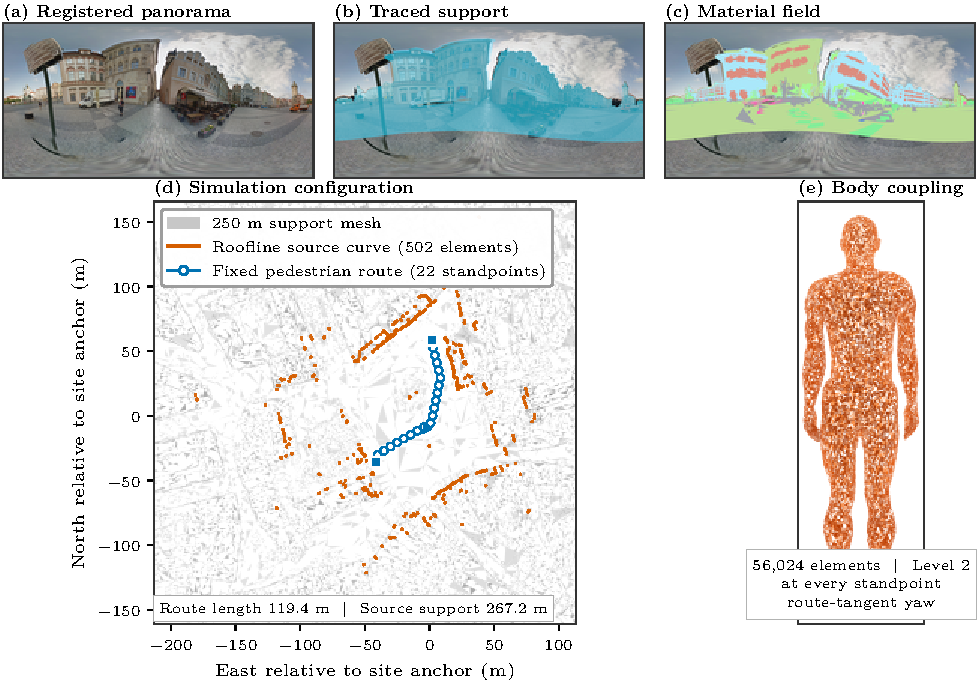
\includegraphics[width=\textwidth]{figures/configuration/configuration.pdf}
  \caption{Simulation configuration at Prague Old Town Square. (a) Registered
  panorama. (b) Traced support mesh. (c) Final transport state after fusion of
  the image evidence. Light solid regions mark atlas interfaces, mid-tone
  diagonal regions mark nonblocking woody vegetation, and dark crosshatched
  regions mark geometric fallback. The redundant fill, pattern, and edge
  encodings are for display only. (d) The 250\,m mesh,
  502 roofline source elements with 267.2\,m total three-dimensional length,
  and the fixed 119.4\,m pedestrian route with 22 standpoints. Light gray is
  the support mesh, orange is the roofline source support, and blue is the
  pedestrian route. (e) The
  56,024-element anatomical surface used at each standpoint, with yaw set by
  the route tangent. Filled squares mark the two registered panorama endpoints,
  and the blue arrow shows the route-tangent yaw at one standpoint. Propagation
  rays are omitted.}
  \label{fig:configuration}
\end{figure*}
